\chapter{Implementation}
In this chapter, we will explain how is our demo game implemented. We will talk about how are data represented and how different modules and third party software libraries work together.

After consideration of the various approaches implemented in games and also proposed efficient solutions to the problem of real-time destructible environment, we decided to try to implement a new approach. We will borrow already tried techniques and put them together in a different way.

Our approach is mostly similar to \emph{Geomod} (described in \cref{sec:common}) with a key differences. Our approach generates Voronoi cell at the point of collision. Then the difference of original mesh and the Voronoi cell is calculated and represents the damaged object. To generate the debris the intersection of original mesh and the Voronoi cell is calculated. This action effectively cuts the object into two or more pieces, all of which are put back into simulation and can be damaged again.

Randomization of the size and shape of a Voronoi cell makes the game look more realistic because it guarantees different result after every collision. The generation of a Voronoi cell takes place in closed cube with its centre at the point of collision. In the cube, in addition to the centre point, random points are generated. The Voronoi cell is the cell of the centre point cut by sides of the cube if necessary.

We also considered implementation based on \emph{A fast method for simulating destruction and the generated dust and debris} (see \cref{sec:edem}). Using the same technology as for our demo game, we set up a cube divided into 439 tetrahedrons. After introducing constraints to hold the elements together, we experienced a drop from default 60fps (set as an upper limit) to 13fps. This result is consistent with results in the article~\cite{edem} and the conclusion is that this approach is not suitable for our work.


\section{Program Structure}
The program is running in three threads (\cref{fig:threads}): the main thread, a thread for subtracting meshes (\cref{sec:subtraction}) and a thread for decomposing triangular mesh into a set of convex shapes (\cref{sec:decomposition}). Both subtraction and decomposition threads communicate only with the main thread, and all communication is done in producer-consumer model. Disregarding the initialization the program runs in following steps:
\begin{enumerate}
\item Perform a step in physics simulation. We measure the time since the last step and leave this task entirely to Bullet physics engine.
\item Handle collisions, see \cref{sec:collisions}.
\item Read user input and then apply correct forces to controlled vehicle.
\item Render current state of objects. In this step, a graphical representation of every object is updated to comply with its rigid body version. Also, the camera has to be properly moved and rotated.
\end{enumerate}

\begin{figure}
        \centering
        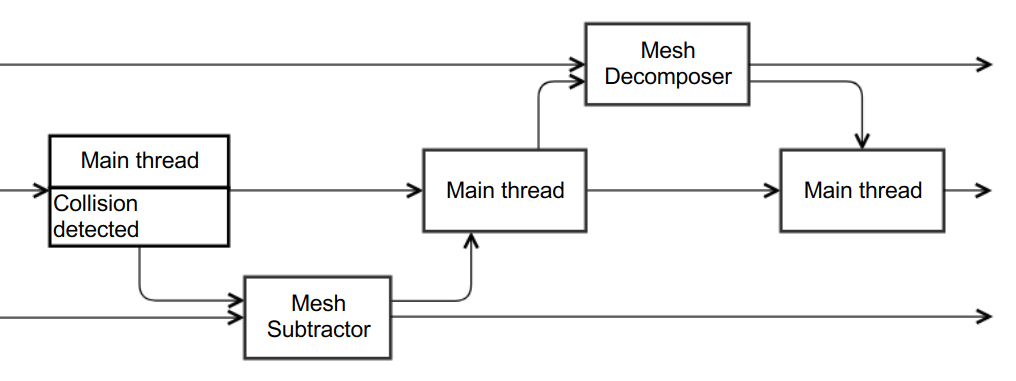
\includegraphics[width=\textwidth]{img/decompositionFlow}
        \caption{Diagram showing multiple threads handling collision event. }
        \label{fig:threads}
\end{figure}



\section{Collision handling}
\label{sec:collisions}
What we get from physics engine after the collision is a reference to two rigid bodies participating in the collision, point of collision and vector of force. For simplification, we will consider only one object, the point of impact and the force.

At first, we need to filter out unwanted collisions (collisions that should not damage the object). Those collisions can be results of an object placed on ground or collisions with not enough force to damage the object. 

For every valid collision, we generate Voronoi cell as described earlier and put meshes of both objects into a task for mesh subtraction thread. After enqueuing all collisions, we check if there are some subtraction results prepared for further use. The result of one subtraction task is a set of meshes that represent new objects. For every mesh, we create a new object, but we do not have its convex decomposition for the physics engine to perform accurate collision detection. Because decomposition can take long, we will create simple temporary collision shape (\eg sphere), a task for decomposition and proceed with simulation. Decomposition is done in its thread, and then the result is returned to the main thread where we in each loop check for decomposed shapes. With the shape ready in the main thread we replace the temporary shape for compound shape made of convex parts.

This process guarantees that we do not wait for either subtraction or decomposition and therefore we can have stable fps in our game. Decomposition is temporarily replaced by a simpler shape which ensures consistent behaviour of new objects (meaning that we can put them into simulation and they do not fall through each other or otherwise not comply with laws of physics). Therefore we need to calculate the difference of meshes in a period of a few frames so it can not be seen that it is lagging behind collisions.


\section{Mesh Subtraction}
\label{sec:subtraction}

\section{Convex Decomposition}
\label{sec:decomposition}



